\chapter{Gráficas del Análisis Exploratorio de datos}
\setcounter{figure}{0} \renewcommand{\thefigure}{A.\arabic{figure}}
\setcounter{table}{0} \renewcommand{\thetable}{A.\arabic{table}}
\begin{subappendices}
\section{Definición de Variables}
	\label{appendix:A}
En este apartado se definen las variables y sus valores que se van a utilizar en este TFM.
\begin{table}[!ht]
	\caption{Nomenclatura de las Variables}
	\centering
	\resizebox{\linewidth}{!}{	\begin{tabular}{|c|c|c|}
			\hline 
			\textbf{	Nombre de la variable} & \textbf{Significado} & \textbf{Valores} \\ 
			\hline 
			CDGENERICO & Indica el código genérico del centro & 
			\begin{minipage}[t]{0.4\textwidth}
				\begin{itemize}
					\item CIMELPR PRSEC = 16
					\item CIMPR SEC = 17
					\item CEPA = 31
					\item CREI = 39
					\item IES = 42
					\item CPR ES = 45
					\item SIES = 47
					\item CPR FPE = 58
					\item CP IFP = 68
					\item CP INF-PRI-SEC = 70
					\item CPR INF-PRI-SEC = 72
					\item CPR PRI-SEC = 73 
				\end{itemize}
			\end{minipage}  \\ 
			\hline 
			CDNATURALEZA & Indica la naturaleza del centro. Centros públicos y privados & 
			\begin{minipage}[t]{0.4\textwidth}
				\begin{itemize}
					\item Público = 1
					\item Privado = 2
				\end{itemize}
			\end{minipage} \\ 
			\hline 
			CDPOSTAL & Código postal del centro &  \\ 
			\hline 
			ITCOMEDOR & Disponibilidad de comedor en el centro &  		\begin{minipage}[t]{0.4\textwidth}
				\begin{itemize}
					\item No = 1
					\item Si = 2
				\end{itemize}
			\end{minipage}\\ 
			\hline 
			ITTRANSPORTE & Disponibilidad de transporte & \begin{minipage}[t]{0.4\textwidth}
				\begin{itemize}
					\item No = 1
					\item Si = 2
				\end{itemize}
			\end{minipage}\\ 
			\hline 
			ITBILINGUE & Disponibilidad de bilingüismo & \begin{minipage}[t]{0.4\textwidth}
				\begin{itemize}
					\item No = 1
					\item Si = 2
				\end{itemize}
			\end{minipage}\\ 
			\hline 
			CD\_NIVEL & Nivel educativo del grupo &    
			\begin{minipage}[t]{0.4\textwidth}
				\begin{itemize}
					\item Bachillerato = 5
					\item Educación Secundaria Obligatoria = 13
					\item Módulos Profesionales = 14
					\item Formación Profesional GM = 15
					\item Formación Profesional GS = 16
				\end{itemize}
			\end{minipage}\\ 
			\hline 
			NM\_CURSO & Curso del nivel educativo del grupo &  
			\begin{minipage}[t]{0.4\textwidth}
				\begin{itemize}
					\item Primero = 1
					\item Segundo = 2
					\item Tercero = 3
					\item Cuarto = 4
				\end{itemize}
			\end{minipage}\\ 
			\hline 
			NM\_UNIDADES & Número de grupos para un determinado nivel y un número de curso &  \\ 
			\hline 
			NM\_ALUMNOS & Número de alumnos para un determinado nivel y numero de curso &  \\ 
			\hline 
			RATIO & Ratio de alumnos por grupo para cada nivel y numero de curso. &  \\ 
			\hline 
			CDSUBDIR & Direccion de Area Territorial (DAT). &  			\begin{minipage}[t]{0.4\textwidth}
				\begin{itemize}
					\item DAT-Norte = 1
					\item DAT-Sur = 2
					\item DAT-Este = 3
					\item DAT-Oeste = 4
					\item DAT-Centro = 5
				\end{itemize}
			\end{minipage}\\ 
			\hline 
			GRUPO\_PREDECIR & Grupo a predecir  &  \\ 
			\hline 
	\end{tabular}}
	
	\label{tab:TablaVariables}
\end{table}

Las variables existentes en las bases de datos originales son: CDGENERICO, CDNATURALEZA, CDPOSTAL, ITCOMEDOR, ITTRANSPORTE, ITBILINGUE, CD\_NIVEL y NM\_CURSO.

El resto de variables se obtienen a partir de las transformaciones correspondientes. Por ejemplo, las variables NM\_UNIDADES NM\_ALUMNOS y GRUPO\_PREDECIR se obtienen de realizar consultas que agrupan por determinados aspectos. Sin embargo, la variable RATIO, que indica la ratio de alumnos para un determinado grupo, se ha obtenido dividiendo la variable de NM\_ALUMNOS entre 30 o 35 (dependiendo del nivel educativo), y este resultado se ha divido entre el número de grupos NM\_GRUPOS para ese nivel educativo. Estos ratios se regulan mediante el \textit{Real Decreto 132/2010, de 12 de febrero, por el que se establecen los requisitos mínimos de los centros que impartan las enseñanzas del segundo ciclo de la educación infantil, la educación primaria y la educación secundaria.} para los niveles de enseñanza de Educación Infantil, Educación Primaria, Educación Secundaria Obligatoria y Bachillerato y el \textit{Real Decreto 1147/2011, de 29 de julio, por el que se establece la ordenación general de la formación profesional del sistema educativo} para los niveles de Formación Profesional. Siendo las ratios los siguientes: 30 para Educación Secundaria Obligatoria y Formación profesional y 35 para Bachillerato.

\section{Análisis exploratorio}

\subsection{Análisis de normalidad}
\label{appendix:AB1}
En primer lugar, se pueden ver la densidad de las variables individualmente de observar a simple vista si cumplen o no con una distribución normal. 

El análisis de normalidad es importante, ya que la falta de normalidad afecta a los modelos que se vayan a utilizar, por ejemplo, a su intervalo de confianza. Dicha falta de normalidad no suele afectar a las predicciones puntuales, pero si a los intervalos o ``errores'' en la predicción.

Para comprobar la normalidad en los datos se utiliza el test de Mardia que es una de las muchas pruebas que se utilizan para dicha comprobación. Existen otras pruebas como el test de Zirkler Henze, Shapiro-Wilk, etc.

Los resultados obtenidos utilizando la prueba de Mardia en el conjunto de datos son los que se pueden observar en la figura \ref{fig:normalidadSUM}

\begin{figure*}[htb]
	\centering
	\caption{Resumen de normalidad de variables. Elaboración propia}
	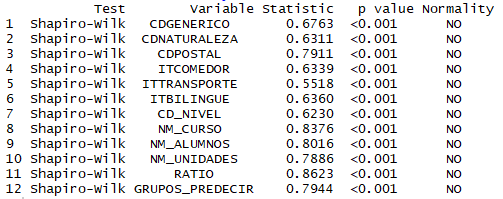
\includegraphics[width=0.8\textwidth]{recursos/ImagenesR/normalidadSUM}
	\label{fig:normalidadSUM}
\end{figure*}
\FloatBarrier


\begin{figure*}[htb]
	\centering
	\caption{Resumen de normalidad de variables. Elaboración propia}
	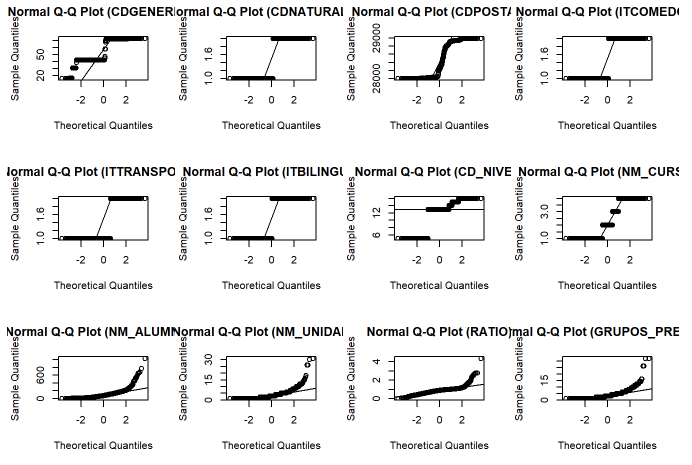
\includegraphics[width=0.8\textwidth]{recursos/ImagenesR/normalidadGRAF}
	\label{fig:normalidadGRAF}
\end{figure*}
\FloatBarrier

Como se puede observar en la figura \ref{fig:normalidadGRAF}, las variables continuas (NM\_ALUMNOS, NM\_UNIDADES, RATIO y GRUPOS\_PREDECIR) son las que más se acercan a la normalidad ya que son cuantitativas, sin embargo no se ajustan a la línea recta teórica que indica el ajuste a la normal.


\begin{figure*}[htb]
	\centering
	\caption{Distribución 1. Elaboración propia}
	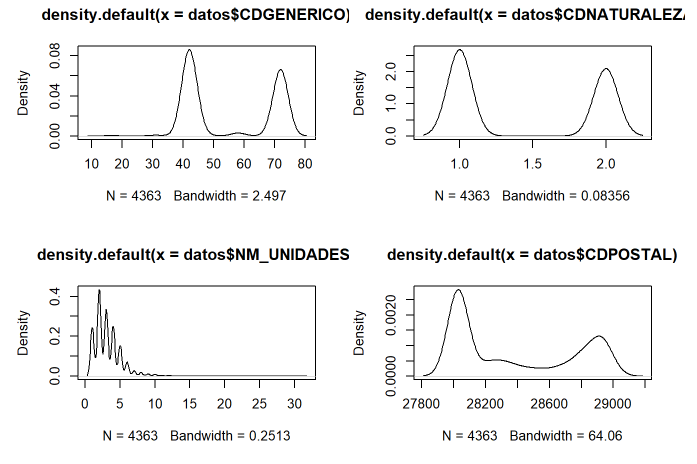
\includegraphics[width=0.8\textwidth]{recursos/ImagenesR/norm1}
	\label{fig:norm1}
\end{figure*}
\FloatBarrier

\begin{figure*}[htb]
	\centering
	\caption{Distribución 2. Elaboración propia}
	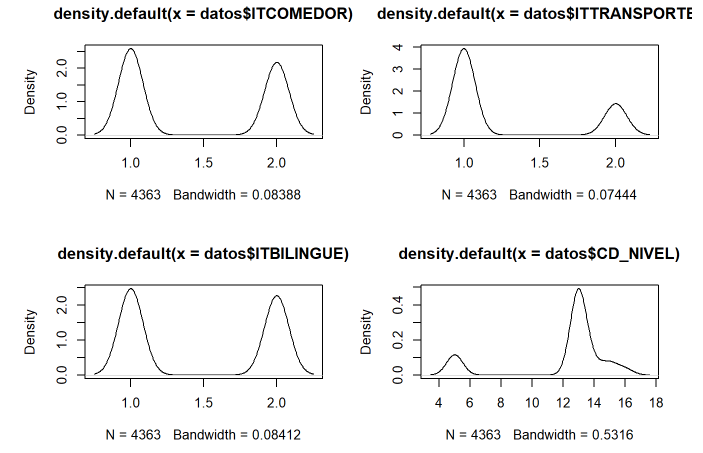
\includegraphics[width=0.8\textwidth]{recursos/ImagenesR/norm2}
	\label{fig:norm2}
\end{figure*}
\FloatBarrier

Las figuras \ref{fig:norm1} y \ref{fig:norm2}, muestran de forma general los valores en los que destacan cada una de las variables. Por ejemplo, viendo la gráfica de densidad de NM\_UNIDADES se puede observar que la media de los grupos por nivel de enseñanza es de 3. Por otro lado la media de alumnos por nivel educativo es de 74.

\begin{figure*}[htb]
	\centering
	\caption{Distribución 3. Elaboración propia}
	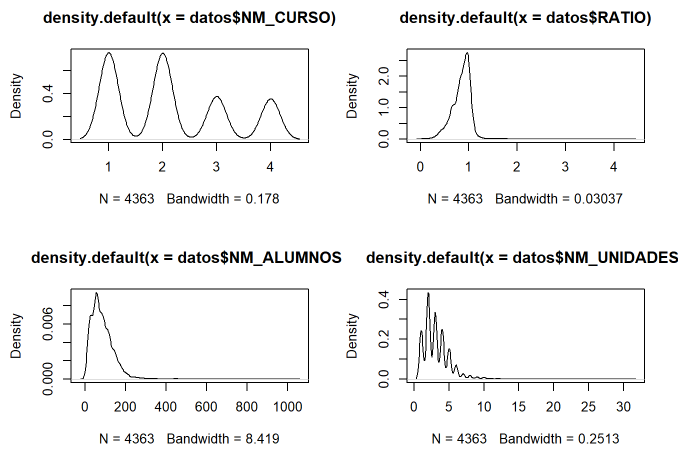
\includegraphics[width=0.8\textwidth]{recursos/ImagenesR/norm3}
	\label{fig:norm3}
\end{figure*}
\FloatBarrier

\begin{figure*}[htb]
	\centering
	\caption{Diagrama de barras 1. Elaboración propia}
	\includegraphics[width=0.8\textwidth]{recursos/ImagenesR/barplot1}
	\label{fig:barplot1}
\end{figure*}
\FloatBarrier

\begin{figure*}[htb]
	\centering
	\caption{Diagrama de barras 2. Elaboración propia}
	\includegraphics[width=0.8\textwidth]{recursos/ImagenesR/barplot2}
	\label{fig:barplot2}
\end{figure*}
\FloatBarrier

Tanto en la figuras \ref{fig:barplot1} y \ref{fig:barplot2} se puede hacer una comparativa sobre los servicios que ofrecen los centros. Se puede observar como la mayoría de centros no tienen transporte. Existe un ligero número de centros que tiene comedor sobre centros que no tienen, de la misma manera ocurre con el bilingüismo. La mayoría de los datos que se tiene son del nivel 13, que corresponde con la Educación Secundaria Obligatoria y la mayoría de estos datos corresponden a centros con el código genérico 42 y 72 (IES y CPR INF-PRI-SEC, respectivamente).

\subsection{Relaciones entre variables}
	\label{appendix:AB2}
Para el estudio de la correlación se utiliza el Coeficiente de Correlación de Pearson (R).

\begin{figure*}[htb]
	\centering
	\caption{Correlación entre variables NM\_ALUMNOS y NM\_GRUPOS. Elaboración propia}
	\label{fig:relacionAlumnGrup}
	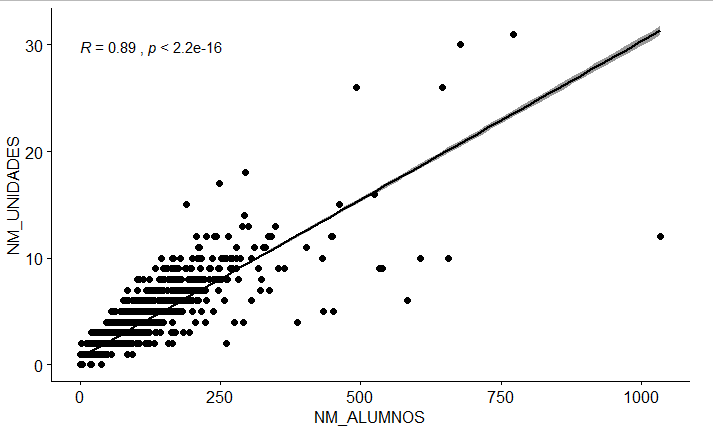
\includegraphics[width=0.6\textwidth]{recursos/ImagenesR/RelacionAlumnGrupos}
	
\end{figure*}
\FloatBarrier

\begin{figure*}[htb]
	\centering
	\caption{Correlación entre variables NM\_UNIDADES y GRUPOS\_PREDECIR. Elaboración propia}
	\label{fig:RelacionGruposYUnidades}
	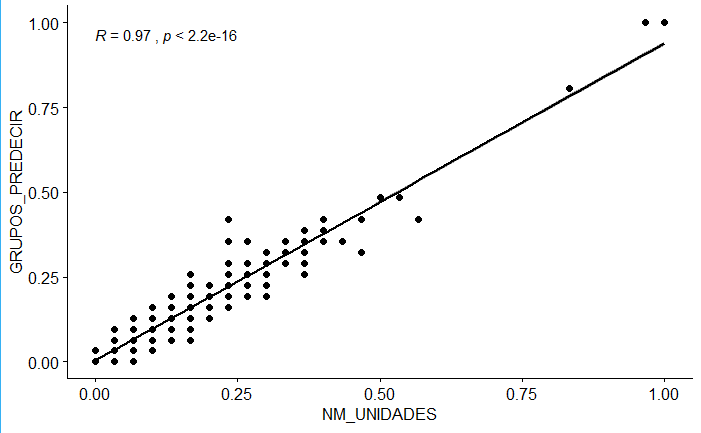
\includegraphics[width=0.6\textwidth]{recursos/ImagenesR/RelacionGruposYUnidades}
	
\end{figure*}
\FloatBarrier

En la figura \ref{fig:RelacionGruposYUnidades} se observa la gran relación (prácticamente lineal) entre las variables NM\_UNIDADES y GRUPOS\_PREDECIR. Esto significa que, si aumenta el valor de una variable, linealmente aumenta el valor de la otra. En la figura \ref{fig:relacionAlumnGrup} existe también una relación lineal, pero no es tan pronunciada.

\section{Selección de Variables}
\subsection{Usando Random Forest}
\label{appendix:AC1}
\begin{figure*}[htb]
	\centering
	\caption{Variables más importantes usando Random Forest. Elaboración propia}
	\label{fig:VarImpRF}
	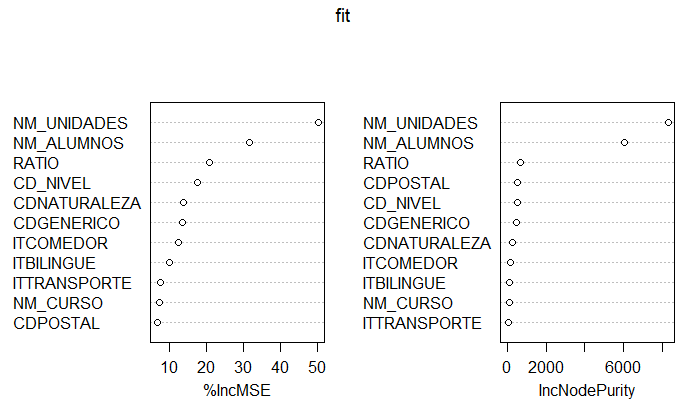
\includegraphics[width=0.6\textwidth]{recursos/ImagenesR/VarImpRF}
	
\end{figure*}
\FloatBarrier
La variable \textbf{IncNodePurity} se la conoce también como la media de decrecimiento de de Gini. El indice de Gini es una ``medida de desorden'' en este caso IncNodePurity tiene el siguiente sentido, a mayor medida, mayor importancia en los modelos creados, puesto que valores próximos a 0 implican un mayor desorden. Por tanto, si computamos la media del "decrecimiento" del indice de Gini cuanto mayor sea esta medida, mas variabilidad aporta a la variable dependiente.

Por otro lado, la variable \textbf{IncMSE} es la media de decrecimiento en la precisión, y es también un indicador sobre la importancia de las variables en el modelo.
\subsection{Regresión Paso a Paso}
\label{appendix:A.C.2}
La regresión por pasos (Stepwise Regression) consiste en añadir o eliminar iterativamente predicadores en el modelo predictivo, con el objetivo de encontrar el subconjunto de los datos que obtengan mayor precisión en el modelo o, dicho de otra forma, reducir el error en la predicción. \cite{kassambara2018}

Existen 3 estrategias para realizar la regresión paso a paso: backward, forward y stepwise.

\subsubsection{Usando Backward Selection}
\begin{figure*}[htb]
	\centering
	\caption{Resultado Backward Selection. Elaboración propia}
	\label{fig:backwardSum}
	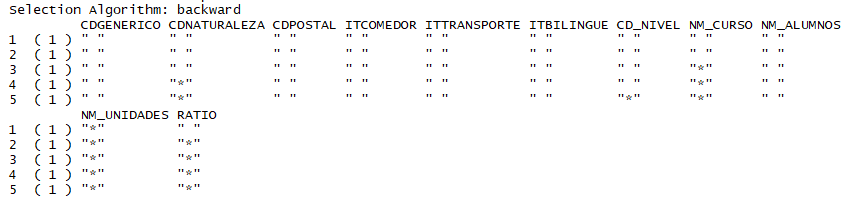
\includegraphics[width=1\textwidth]{recursos/ImagenesR/backwardSum}
	
\end{figure*}
\FloatBarrier

Los asteriscos en los resultados indican los predictores que se deben tomar para realizar el modelo. En este caso se necesitan las variables CD\_NATURALEZA, CD\_NIVEL, NM\_CURSO, NM\_UNIDADES y RATIO.

\begin{figure*}[htb]
	\centering
	\caption{Gráfico Backward Selection. Elaboración propia}
	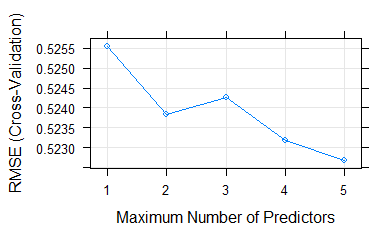
\includegraphics[width=0.6\textwidth]{recursos/ImagenesR/backward}
	\label{fig:backward}
\end{figure*}
\FloatBarrier

En la figura \ref{fig:backward} se puede observar como la mejor precision se obtiene utilizando los 5 predictores de la figura \ref{fig:backwardSum}.

\subsubsection{Usando Stepwise Selection}
\begin{figure*}[htb]
	\centering
	\caption{Resultado Stepwise Selection. Elaboración propia}
	\label{fig:seqSum}
	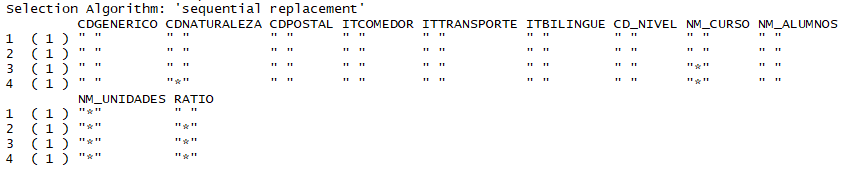
\includegraphics[width=1\textwidth]{recursos/ImagenesR/seqSum}
	
\end{figure*}
\FloatBarrier

Nuevamente los asteriscos de la figura \ref{fig:seqSum} indican aquellos predictores que deben utilizarse, en este caso son: CD\_NATURALEZA, NM\_CURSO, NM\_UNIDADES y RATIO.

\begin{figure*}[htb]
	\centering
	\caption{Gráfico Stepwise Selection. Elaboración propia}
	\label{fig:seq}
	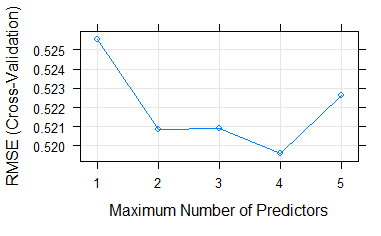
\includegraphics[width=0.6\textwidth]{recursos/ImagenesR/seq}
	
\end{figure*}
\FloatBarrier

En la figura \ref{fig:seq} se puede observar como la mayor precisión (menor valor de RMSE) se obtiene utilizando 4 variables.


\subsubsection{Usando Forward Selection}
\begin{figure*}[htb]
	\centering
	\caption{Resultado Forward Selection. Elaboración propia}
	\label{fig:fordwardSum}
	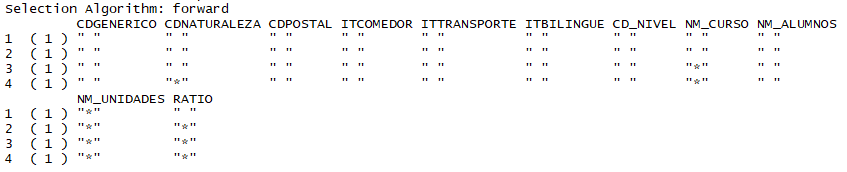
\includegraphics[width=1\textwidth]{recursos/ImagenesR/fordwardSum}
\end{figure*}
\FloatBarrier

En los resultados de la figura \ref{fig:fordwardSum} se puede observar como nuevamente se tienen en cuenta las variables CD\_NATURALEZA, NM\_CURSO, NM\_UNIDADES y RATIO.

\begin{figure*}[htb]
	\centering
	\caption{Gráfico Forward Selection. Elaboración propia}
	\label{fig:fordward}
	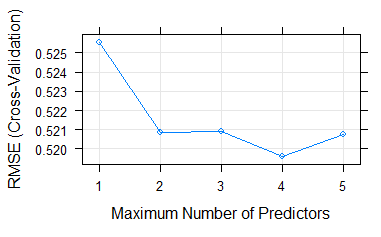
\includegraphics[width=0.6\textwidth]{recursos/ImagenesR/fordward}
\end{figure*}
\FloatBarrier

Al igual que en la estrategia de ``Stepwise'', se ha obtenido el mejor resultado de RMSE utilizando 4 variables. Estas variables son las obtenidas en el resultado de la figura \ref{fig:fordwardSum}.	

Como conclusión se puede obtener que tanto usando el algoritmo de Random Forest como las varias estrategias del algoritmo de Regresión paso a paso, se han seleccionado mayoritariamente 4 variables a destacar en la utilización de un modelo y son las siguientes ordenadas por importancia: NM\_UNIDADES, NM\_ALUMNOS, RATIO, CD\_NIVEL y CD\_NATURALEZA. 
\end{subappendices}



\chapter{Análisis Predictivo}
\setcounter{figure}{0} \renewcommand{\thefigure}{B.\arabic{figure}}
\setcounter{table}{0} \renewcommand{\thetable}{B.\arabic{table}}

Como ya se ha comentado en el diseño, a la hora de realizar un análisis predictivo utilizando técnicas de aprendizaje supervisado, es necesario dividir los datos en un 70\% para entrenar el modelo y el otro 30\% para probarlo.

Una vez que se han dividido los datos, se realiza una comparación con los modelos seleccionados. Se recuerda que los modelos utilizados a grandes rasgos han sido las redes neuronales, los k-vecinos más cercanos, los bosques aleatorios (Random Forest), la regresión logística, el soporte de vectores de máquinas y los arboles de decisión.

Estos modelos comentados a su vez tienen una serie de algoritmos distintos tanto para crear modelos de clasificación como para crear modelos de regresión. En este caso, debido a que es la predicción de datos continuos, se va a utilizar la regresión.

Los algoritmos que se han utilizado para cada modelo seleccionado son los siguientes: K-Vecinos Cercanos (kknn), Redes neuronales bayesianas regularizadas (brnn), bosques aleatorios (rf), Máquinas de soporte de vectores con núcleo lineal (svmLinear), Árbol Modelo (M5) y el Elasticnet (enet) en la Regresión Lineal.

\begin{subappendices}
	\label{appendix:B}
\section{Comparación de Modelos}

Para realizar la comparación de modelos se utiliza una técnica del paquete Caret, donde se realiza un entrenamiento con los datos usando todos los modelos comentados en el apartado 4.3.4 del capítulo de Diseño de la Investigación. 

Para realizar la comparación de modelos se realiza una medición no solo en la precisión de estos sino también el tiempo transcurrido en entrenar el propio modelo.

Todos los modelos se entrenan usando los mismos parámetros, de esta forma ninguno de ellos resulta favorecido. Obviamente los resultados de los modelos dependen de dichos parámetros. Realizando combinaciones de estos parámetros se obtienen una serie de resultados para cada modelo al final se selecciona el mejor resultado para cada modelo y estos resultados son los que se compararan con el resto de modelos.

Ademas de los modelos comentados, se han entrenado dichos modelos, pero teniendo en cuenta las 5 variables seleccionadas por los algoritmos de selección de variables. A continuación se muestran en la siguiente tabla \ref{tab:ComparacionModelos} los modelos, su predicción y sus tiempos.

\begin{table}[!ht]
	\caption{Tabla comparación modelos (precisión y tiempo)}
	\label{tab:ComparacionModelos}
	\centering
	\begin{tabular}{|c|c|c|}
		\hline 
		Modelos & Precisión & Tiempo Entrenamiento \\ 
		\hline 
		Redes neuronales (NN) & 0.5236718 & 52.10 \\ 
		\hline 
		Redes neuronales - 5 variables (NN2) & 0.5242227 & 29.38 \\ 
		\hline 
		K-Vecinos Cercanos (KKNN) & 0.6468044 & 16.69 \\ 
		\hline 
		K-Vecinos Cercanos - 5 variables (KKNN2) & 0.5982330 & 14.86 \\ 
		\hline 
		Random Forest (RF) & 0.5264411 & 947.03 \\ 
		\hline 
		Random Forest - 5 variables (RF2) & 0.5577621 & 515.49 \\ 
		\hline 
		Vector de Máquinas Soporte (SVM) & 0.5336122 & 37.93 \\ 
		\hline 
		Vector de Máquinas Soporte - 5 variables (SVM2) & 0.5409171 & 21.22 \\ 
		\hline 
		Regresión Linear (enet) & 0.5256446 & 2.78 \\ 
		\hline 
		Regresión Linear - 5 variables (enet2) & 0.5245138 & 2.13 \\ 
		\hline 
		Árbol de decisión (xgbTree) & 0.5146266 & 247.83 \\ 
		\hline 
		Árbol de decisión -5 variables (xgbTree2) & 0.5311688 & 228.45 \\ 
		\hline 
	\end{tabular} 
\end{table}
\FloatBarrier

A continuación, se muestra gráficamente los resultados de la tabla anterior.

\begin{figure*}[htb]
	\centering
	\caption{Comparación Modelos y Precisión. Elaboración propia}
	\label{fig:ComparacionModelosII}
	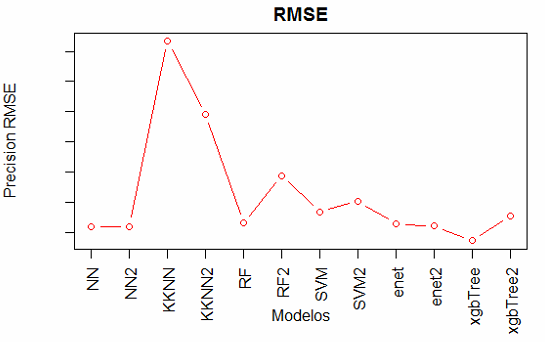
\includegraphics[width=0.8\textwidth]{recursos/ImagenesR/ComparacionModelos2}
\end{figure*}
\FloatBarrier

\begin{figure*}[htb]
	\centering
	\caption{Comparación Modelos y Tiempo en Entrenar. Elaboración propia}
	\label{fig:ComparacionModelosTiempo}
	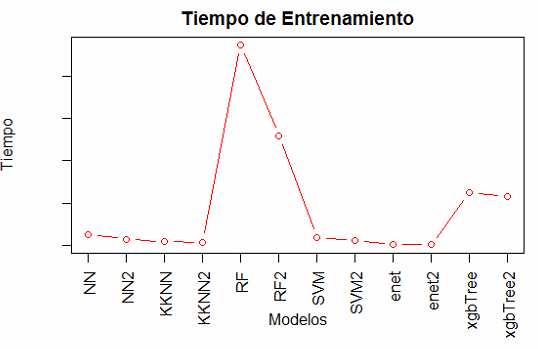
\includegraphics[width=0.8\textwidth]{recursos/ImagenesR/ComparacionModelosTiempo}
\end{figure*}
\FloatBarrier
\end{subappendices}

\chapter{Sistema de Explotación de la Consejería de Educación e Investigación}
\setcounter{figure}{0} \renewcommand{\thefigure}{C.\arabic{figure}}
\setcounter{table}{0} \renewcommand{\thetable}{C.\arabic{table}}
	\label{appendix:C}
En este apartado se van a mostrar una serie de imágenes de la aplicación de explotación de datos de la Consejería de Educación e Investigación. Concretamente se van a mostrar dos Cuadros de Mandos.

En primer lugar, se ha realizado un Cuadro de Mando relativo a los centros sostenidos con fondos públicos. En este cuadro de mando se muestran aspectos como el número de alumnos matriculados, el numero de unidades, el porcentaje de centros públicos y concertados, la nacionalidad de los alumnos, el sexo, etc. Véase la figura \ref{fig:CentrosResumenI}

Existe un filtro, donde se puede seleccionar los parámetros de la búsqueda. Entre estos filtros se encuentran los siguientes: año, área territorial, municipio, distrito, centro educativo y nivel educativo.

\begin{figure*}[htb]
	\centering
	\caption{Cuadro de Mandos de Centros I. Elaboración propia}
	\label{fig:CentrosResumenI}
	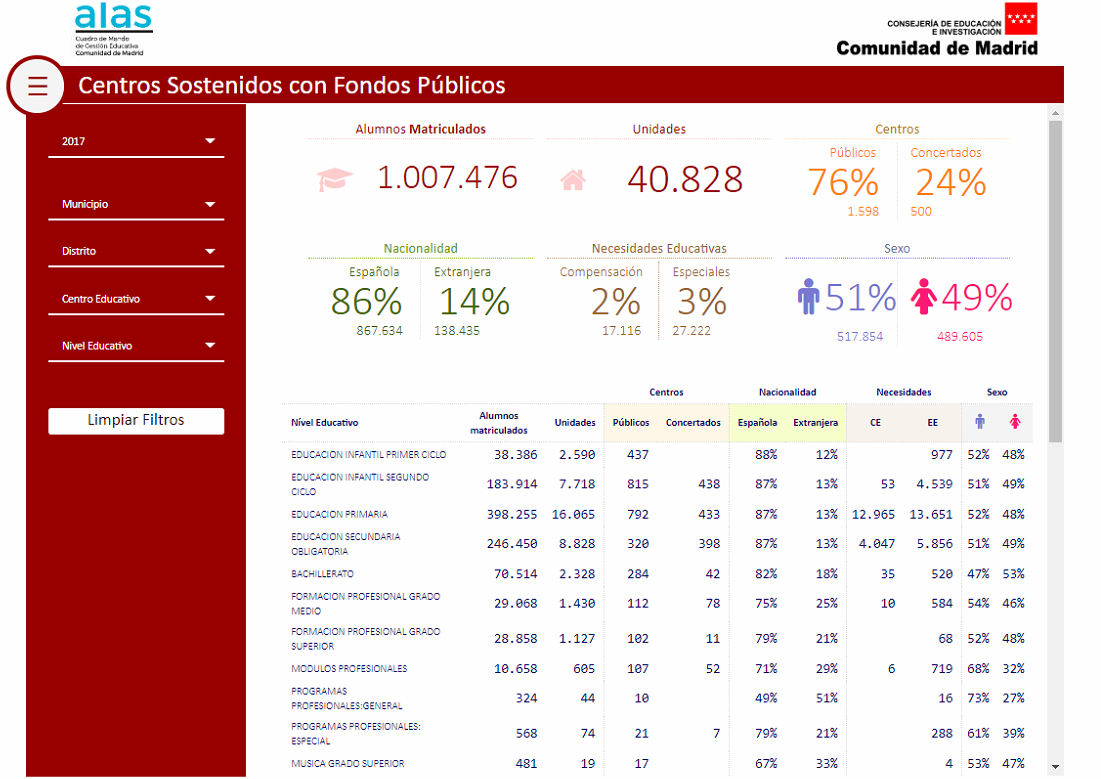
\includegraphics[width=1\textwidth]{recursos/CentrosResumenI}
\end{figure*}

En la figura \ref{fig:CentrosResumenII} se ha realizado una búsqueda sobre el nivel educativo de E.S.O. en el centro educativo de ``Jose Luis Sampedro'', que se encuentra en Tres Cantos (DAT-Norte).
\begin{figure*}[htb]
	\centering
	\caption{Cuadro de Mandos de Centros II. Elaboración propia}
	\label{fig:CentrosResumenII}
	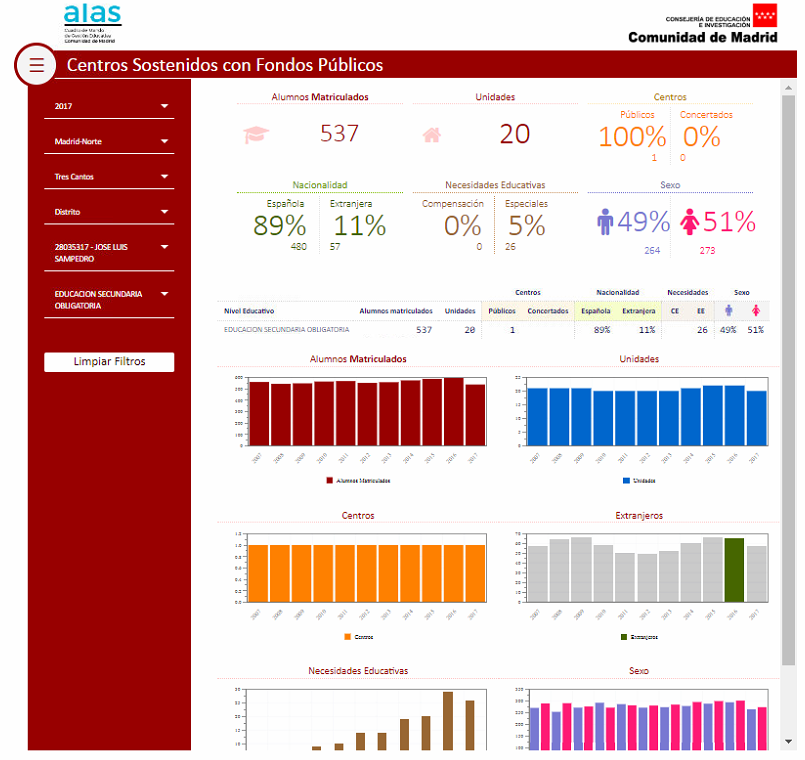
\includegraphics[width=1\textwidth]{recursos/CentrosResumenII}
\end{figure*}
\FloatBarrier

Otro cuadro de mandos realizado ha sido el de ausencias de alumnados en centros de Secundaria, Bachillerato y FP.

En este cuadro de mando aparecen las faltas de asistencias totales, el número de retrasos, el porcentaje sobre el total entre faltas y retrasos, el porcentaje de faltas y retrasos justificados. Se muestra un histograma también sobre el número de faltas y retrasos y los días de la semana.

\begin{figure*}[htb]
	\centering
	\caption{Cuadro de Mandos de Ausencias de Alumnado I. Elaboración propia}
	\label{fig:FaltasAsistenciaI}
	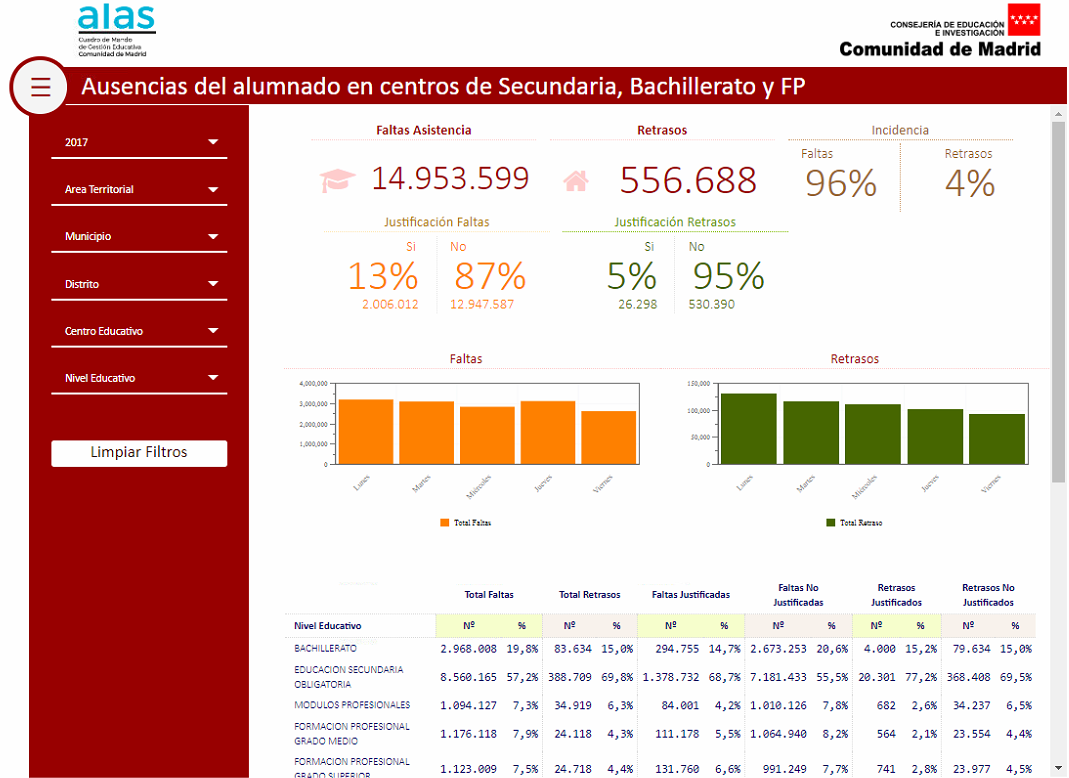
\includegraphics[width=1\textwidth]{recursos/FaltasAsistenciaI}
\end{figure*}
\FloatBarrier

En la figura \ref{fig:FaltasAsistenciaII} se filtra la búsqueda por el municipio de Parla (DAT-Sur), para el año 2017.

\begin{figure*}[htb]
	\centering
	\caption{Cuadro de Mandos de Ausencias de Alumnado II. Elaboración propia}
	\label{fig:FaltasAsistenciaII}
	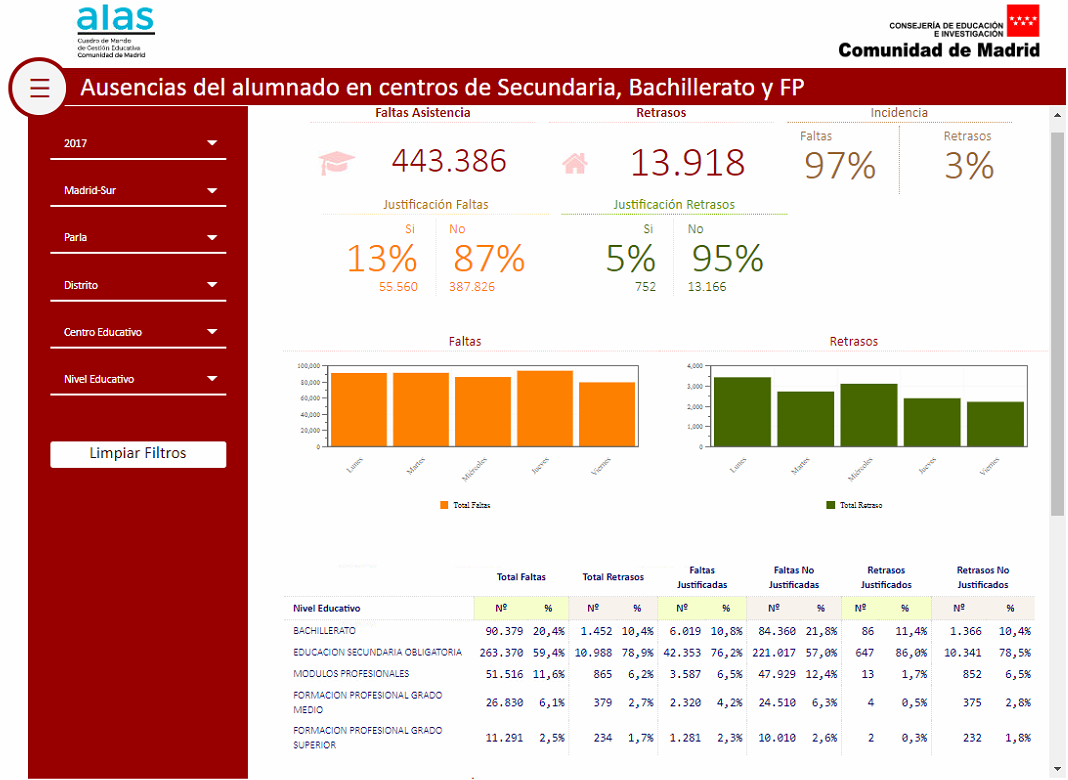
\includegraphics[width=1\textwidth]{recursos/FaltasAsistenciaII}
\end{figure*}
\FloatBarrier

Además, aunque no se haya creado cuadro de mandos, se ha realizado cubos OLAP de las unidades, los centros, las faltas de asistencia, las minorías étnicas, etc. En este caso se va a mostrar en la siguiente ilustración \ref{fig:STPivotUnidades} el cubo OLAP relativo a las unidades.

\begin{figure*}[htb]
	\centering
	\caption{Cubo OLAP de Unidades. Elaboración propia}
	\label{fig:STPivotUnidades}
	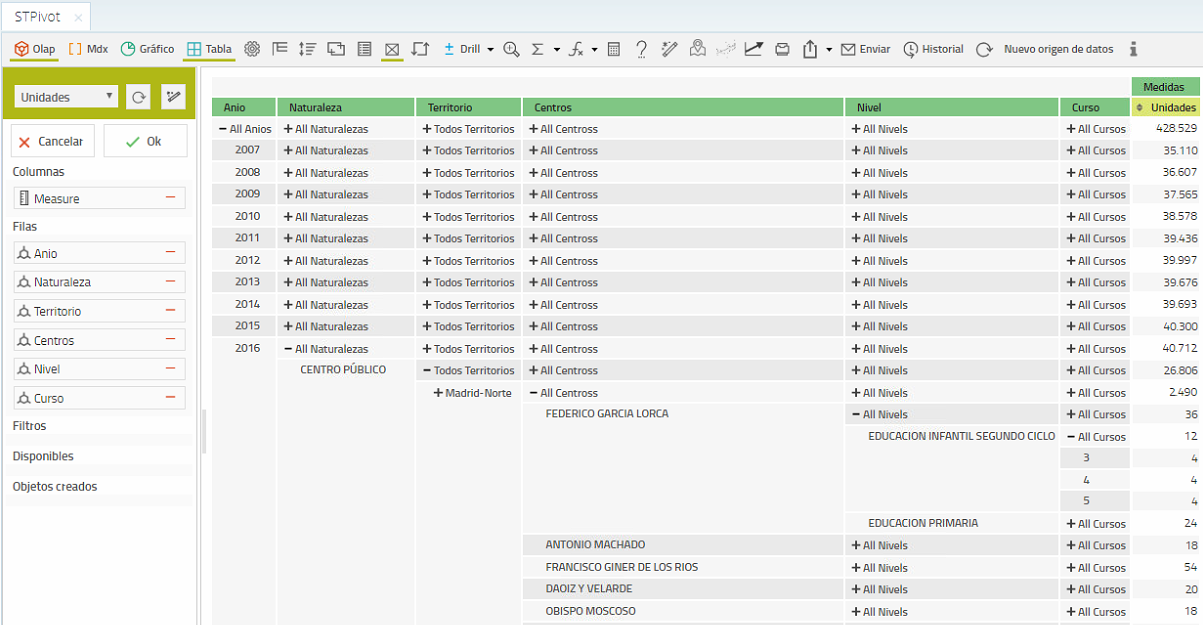
\includegraphics[width=1\textwidth]{recursos/STPivotUnidades}
\end{figure*}
\FloatBarrier




